\documentclass[a4paper,12pt]{article}

%%% Работа с русским языком
\usepackage{cmap}					% поиск в PDF
\usepackage{mathtext} 				% русские буквы в формулах
\usepackage[T2A]{fontenc}			% кодировка
\usepackage[utf8]{inputenc}			% кодировка исходного текста
\usepackage[english,russian]{babel}	% локализация и переносы
\usepackage{xcolor}
\usepackage{hyperref}
 % Цвета для гиперссылок
\definecolor{linkcolor}{HTML}{799B03} % цвет ссылок
\definecolor{urlcolor}{HTML}{799B03} % цвет гиперссылок

\hypersetup{pdfstartview=FitH,  linkcolor=linkcolor,urlcolor=urlcolor, colorlinks=true}

%%% Дополнительная работа с математикой
\usepackage{amsfonts,amssymb,amsthm,mathtools} % AMS
\usepackage{amsmath}
\usepackage{icomma} % "Умная" запятая: $0,2$ --- число, $0, 2$ --- перечисление

%% Номера формул
%\mathtoolsset{showonlyrefs=true} % Показывать номера только у тех формул, на которые есть \eqref{} в тексте.

%% Шрифты
\usepackage{euscript}	 % Шрифт Евклид
\usepackage{mathrsfs} % Красивый матшрифт

%% Свои команды
\DeclareMathOperator{\sgn}{\mathop{sgn}}

%% Перенос знаков в формулах (по Львовскому)
\newcommand*{\hm}[1]{#1\nobreak\discretionary{}
{\hbox{$\mathsurround=0pt #1$}}{}}
% графика
\usepackage{graphicx}
\graphicspath{{pictures/}}
\DeclareGraphicsExtensions{.pdf,.png,.jpg}
\author{Бурмашев Григорий, БПМИ-208}
\title{}
\date{\today}
\begin{document}
\section*{Задание 3}
Посмотрим на первые строчки треугольника паскаля:

\begin{center}
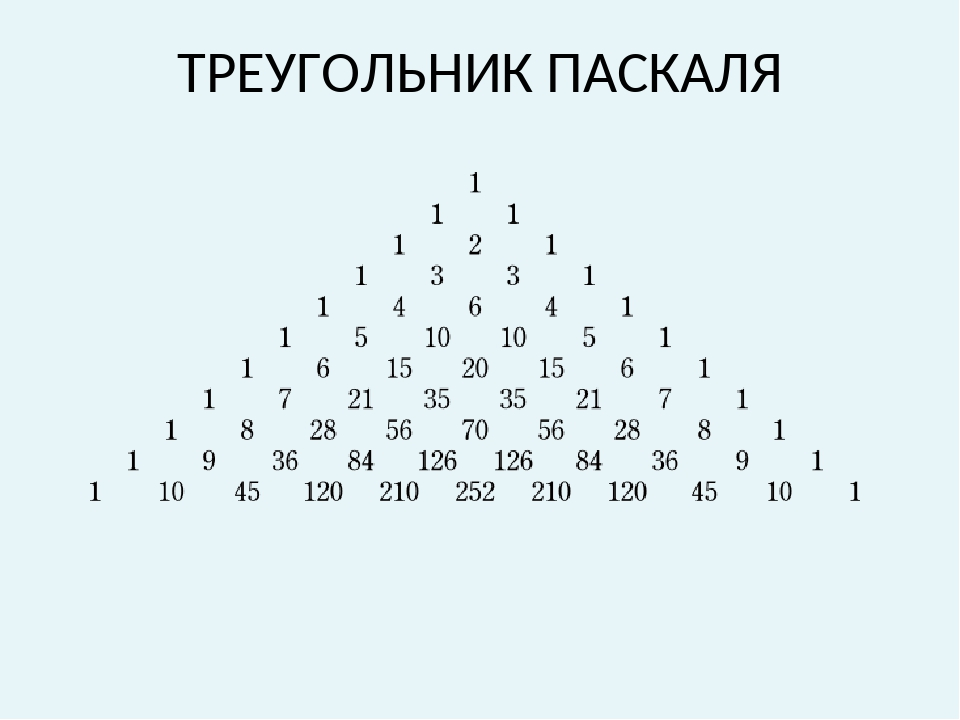
\includegraphics[scale=0.2]{img8.jpg}
\end{center}
Можем найти закономерность, назовем искомую сумму $S_n$, тогда для маленьких $n$:
\[
S_1 = 2
\]
\[
S_2 = 4
\]
\[
S_3 = 8
\]
\[
S_4 = 16
\]
Предположим, что формула задается в виде $2^n$. Для $n$ от 1 до 4 это выполняется. Предположим, что выполняется для $n$, тогда для $n + 1$:

Мы знаем, что в $n + 1$ строке каждое слагаемое является суммой двух из $n$ строки(по определению), при этом каждый элемент из $n$ строки возникает в $n + 1$ 2 раза, значит:
\[
S_{n + 1} = 2 \cdot S_n = 2^{n + 1}
\]
\begin{center}
\textbf{Ответ: } $2^n$
\end{center}
\end{document}

